\documentclass[A4paper, 12pt, oneside]{book}%begin
\usepackage[margin=1in]{geometry}
\usepackage[czech]{babel}
\usepackage[utf8]{inputenc}
\usepackage[pdftex]{graphicx}
\usepackage{tabularx}
\usepackage{enumitem}
\usepackage{epstopdf}
\usepackage{setspace}
\usepackage{csquotes}
\usepackage{amsmath, amssymb, amsthm}
\DeclareMathOperator{\tg}{tg}
\DeclareMathOperator{\arctg}{arctg}
\usepackage[inline]{asymptote}
\usepackage{esdiff, icomma, subcaption}
\usepackage{blindtext}
\usepackage[toc]{appendix}
\renewcommand{\appendixname}{Přílohy}
\renewcommand{\appendixtocname}{Přílohy}

\usepackage{listings}
\lstdefinestyle{mystyle}{
    breakatwhitespace=false,         
    breaklines=true,                 
    basicstyle=\footnotesize,
}
\lstset{style=mystyle}


\usepackage[backend=biber, url=true, sorting=none]{biblatex}
\usepackage{url}
\addbibresource{soc.bib}

\newcommand{\B}[1]{\textbf{#1}}
\newcommand{\C}[1]{\textsc{#1}}
\renewcommand{\S}[1]{\textsc{#1}}
\newcommand{\I}[1]{\textit{#1}}
\newcommand{\mB}[1]{\mathbf{#1}}
\newcommand{\ap}{{\,\prime}}
\newcommand{\abs}[1]{\lvert #1 \,\rvert}

\setstretch{1.3}
\renewcommand*\contentsname{Obsah}
\renewcommand{\theequation}{\arabic{equation}}%end

\begin{document}
\topskip0pt
\begin{center}
	{\LARGE \B{\S{Středoškolská odborná činnost}}} \\
	{\large \B{{Obor č. 2: Fyzika}}}
\end{center}
\vfill
\begin{center}
	{\Huge \B{Mechanika rodin planetek \\ s~aplikací na rodinu Eunomia}}
\end{center}
\vfill
{\large \bfseries Adam Křivka \\
	Jihomoravský kraj \hfill Brno 2018}

\newpage

\begin{center}
	{\LARGE \B{\S{Středoškolská odborná činnost}}} \\
	{\large \B{{Obor č. 2: Fyzika}}}
\end{center}
\vfill
\begin{center}
	{\Huge \B{Mechanika rodin planetek \\ s~aplikací na rodinu Eunomia}}

	{\Huge \B{Asteroid families mechanics \\ with application to the family Eunomia}}
\end{center}
\vfill
\begin{tabularx}{\textwidth}{lX}
	{\bfseries Autoři:} & Adam Křivka \\
	{\bfseries Škola:} & Cyrilometodějské gymnázium a střední odborná škola pedagogická Brno, Lerchova 63, 602 00 Brno \\
	{\bfseries Kraj:} & Jihomoravský kraj \\
	{\bfseries Konzultant:} & doc. Mgr. Miroslav Brož, Ph.\,D.
\end{tabularx}

\

\noindent Brno 2018

\newpage

{\large \bfseries Prohlášení}

Prohlašuji, že jsem svou práci SOČ vypracoval/a samostatně a použil/a jsem pouze prameny a literaturu uvedené v~seznamu bibliografických záznamů.

Prohlašuji, že tištěná verze a elektronická verze soutěžní práce SOČ jsou shodné. 

Nemám závažný důvod proti zpřístupňování této práce v~souladu se zákonem č. 121/2000 Sb., o~právu autorském, o~právech souvisejících s~právem autorským a o~změně některých zákonů (autorský zákon) ve znění pozdějších předpisů. 

\

V~Brně dne \today\ \dotfill \hspace{10mm}

\newpage

{\large \bfseries Poděkování}

\newpage

{\large \bfseries Anotace}

{\large \bfseries Klíčová slova}

{\large \bfseries Annotation}

{\large \bfseries Keywords}

\newpage

\tableofcontents

\newpage

\chapter{Úvod do nebeské mechaniky}
TODO: Úvod
\vspace{40mm}
\section{Pohybové rovnice}
Pohybová rovnice je matematicky zapsaný fyzikální vztah, který popisuje možné pohyby těles v~daném prostředí \cite{wiki:eqm}. Řešením pohybové rovnice je funkce, popisující polohu a rychlost každého zkoumaného tělesa v~závislosti na čase. Přitom potřebujeme znát počáteční podmínky --- polohy a rychlosti těles na začátku. Pohybová rovnice bývá ve tvaru diferenciální rovnice, což je rovnice, která vyjadřuje vztah mezi nějakou funkcí a jejími derivacemi, což je okamžitá změna hodnoty funkce při velmi malé změně argumentu, v~našem případě času. 

V~následující části se pokusíme nalézt řešení pohybové rovnice pro tělesa ve sluneční soustavě. Zákony, jimiž se budou naše tělesa řídit, jsou Newtonův gravitační zákon a Newtonovy pohybové zákony, které byly poprvé definovány Isaacem Newtonem (1642--1726) již v~roce 1687.
\subsection{Rovnice pro dvě tělesa} \label{sec:2body}
Omezme se nyní na dvě tělesa a nalezněme řešení tzv.\ problému dvou těles --- Keplerovy úlohy. To znamená, že se pokusíme odvodit funkci, popisující polohu a rychlost obou těles v~závisloti na čase. 

Nacházíme se v~inerciální vztažné soustavě, což je taková vztažná soustava, kde platí první Newtonův zákon. Jako bod v~klidu si zvolme těžiště soustavy. Pro síly působící na obě tělesa podle Newtonova gravitačního zákona a druhého a třetího pohybového zákona platí
\begin{align} 
	\vec{F}_1 &= +G\frac{m_1m_2}{\abs{\vec{r}}^3}\vec{r} = m_1\vec{a}_1\,, \label{eq:newton1} \\
	\vec{F}_2 &= -G\frac{m_1m_2}{\abs{\vec{r}}^3}\vec{r} = m_2\vec{a}_2\,, \label{eq:newton2}
\end{align}
kde $G$ označuje gravitační konstantu, $m_1$, $m_2$ hmotnosti zkoumaných těles, $\vec{a}_1$, $\vec{a}_2$ vektory zrychlení těles (tj.\ druhé derivace polohových vektorů $\vec{r}_1$, $\vec{r}_2$ podle času) a $\vec{r}$ vektor udávající vzájemnou polohu těles, definovanou jako $\vec{r} \equiv \vec{r}_2 - \vec{r}_1$. Sečtením obou rovnic dostáváme
\begin{equation} \label{eq:mr0}
	\vec{F}_1 + \vec{F}_2 = m_1\vec{a_1} + m_2\vec{a_2} = \vec{0}\,.
\end{equation}
Vektor popisující polohu těžiště soustavy je $\vec{R} \equiv \frac{m_1\vec{r}_1 + m_2\vec{r}_2}{m_1 + m_2}$. Jeho druhou derivací podle času dostáváme zrychlení
\begin{equation*}
	\diff[2]{\vec{R}}{t} = \frac{m_1\vec{a_1} + m_2\vec{a_2}}{m_1+m_2} = \vec{0}\,,
\end{equation*}
které se podle \eqref{eq:mr0} rovná nule, takže se těžiště soustavy pohybuje konstantní rychlostí.
\newpage
Nyní se však přesuňme do soustavy neinerciální, kde je první z~těles (běžně to hmotnější) nehybné. Označme $\vec{a}\equiv\vec{a}_2-\vec{a}_1$ zrychlení druhého tělesa vzhledem k~prvnímu. Po pokrácení $m_1$ a $m_2$ můžeme odečíst upravenou rovnici~\eqref{eq:newton1} od upravené rovnice~\eqref{eq:newton2}, čímž dostaneme
\begin{align}
	\nonumber \vec{a}_2 - \vec{a}_1 = -Gm_1\frac{\vec{r}}{\abs{\vec{r}}^3}-Gm_2\frac{\vec{r}}{\abs{\vec{r}}^3}\,, \\
	\nonumber \vec{a} = -G(m_1+m_2)\frac{\vec{r}}{\abs{\vec{r}}^3}\,, \\
		\diff[2]{\vec{r}}{t} + G(m_1+m_2)\frac{\vec{r}}{\abs{\vec{r}}^3} = \vec{0}\,.	
\end{align}
Často ještě definujeme gravitační paramter soustavy $\mu\equiv G(m_1+m_2)$.

I~přesto, že tato diferenciální rovnice ještě není ve své konečné podobě vhodné k~tomu, abychom z~ní odvodili následující vztah, prozradíme, že je jím funkce v~polárních souřadnicích, popisující vzdálenost těles $r\equiv\abs{\vec{r}}$ v~závisloti na úhlu $\theta$, který svírá přímka procházející oběma tělesy a nějaká zvolená referenční přímka, přesné odvození viz~\cite{murray99}.
\begin{equation} \label{eq:polar}
	r(\theta)=\frac{p}{1+e\cos{(\theta-\omega)}}\,.
\end{equation}
Vztah \eqref{eq:polar} je obecným předpisem kuželosečky --- hyperboly, paraboly, elipsy nebo kružnice; pro naše účely se zaměřme na případ elipsy, kdy se v~jednom z~jejích ohnisek nachází centrální těleso.

Veličina $p$ označuje parametr elipsy, jehož velikost je určena hodnotou $\mu$ a veličinou~$h=|\vec{h}| \equiv \vec{r}\times\diff{\vec{r}}{t}={\rm konst.}$\footnote{což je \uv{něco jako} moment hybnost systému na jednotku hmotnosti $\mu$. Vycházíme z~předpokladu, že gravitační síly (né nutně splňující Newtonův gravitační zákon) mezi tělesy jsou stejně velké a působí proti sobě, tedy $\vec{r}\times\vec{a}=\vec{r}\times\diff[2]{\vec{r}}{t}=0$, z~čehož integrací vzhledem k~času můžeme vyvodit právě $\vec{r}\times\diff{\vec{r}}{t}=\vec{h}$, kde $\vec{h}$ je vektor kolmý na rovinu obýhání těles.}, kde $\times$ značí vektorový součin, jako
\begin{align}
	p=\frac{h^2}{\mu}\,,
\end{align}
a pro který dále platí vztah
\begin{align}
	p=\frac{b^2}{a}\,,
\end{align}
kde $a$ označuje délku hlavní poloosy, což je úsečka spojující střed elipsy s~jedním z~průsečíků elipsy s~hlavní osou --- přímkou spojující ohniska, a $b$ označuje délku vedlejší poloosy, což je úsečka spojující střed elipsy s~průsečíkem elipsy s~přímkou kolmou na hlavní poloosu a procházející středem elipsy --- vedlejší osou (viz obrázek~\ref{fig:elip}).

Dále $e$, resp.\ $\omega$ jsou integrační konstanty a nazývají se excentricita, resp.\ argument pericentra. Pro excentricitu platí vztah
\begin{figure}
	\centering
	\begin{asy}
		size(12cm);

		marker mark1 = marker(scale(circlescale*2)*unitcircle, Fill);

		real a = 1.5;
		real b = 1;
		real omega = 25;
		real s = 1.5;

		draw(rotate(omega)*ellipse((0,0), a, b));

		draw(rotate(omega)*(a,0)--rotate(omega)*(-a,0));
		draw(rotate(omega)*(0,-b)--rotate(omega)*(0,b));
		draw((0,0), mark1);

		draw(rotate(omega)*(a,0), mark1);
		draw(rotate(omega)*(-a,0), mark1);
		label("{\footnotesize pericentrum}", rotate(omega)*(a,0), rotate(omega)*E);
		label("{\footnotesize apocentrum}", rotate(omega)*(-a,0), rotate(omega)*W);

		real F = sqrt((a-b)*(a+b));
		draw(rotate(omega)*(F,0), mark1);
		draw(rotate(omega)*(-F,0), mark1);
		label("$F_1$", rotate(omega)*(F,0), S);
		label("$F_2$", rotate(omega)*(-F,0), S);

		draw(rotate(omega)*brace((0,0), (a,0)));
		label("$a$", rotate(omega)*(a/2,0), rotate(omega)*4N);

		draw(brace((0,0), rotate(omega)*(0,b)));
		label("$b$", rotate(omega)*(0, b/2), rotate(omega)*3W);

		draw((0,0)--scale(s)*(a,0), arrow=EndArrow);
		//draw((0,0)--scale(s)*(0,b), arrow=EndArrow);
		label("{\footnotesize referenční směr}", scale(s)*(a,0), S);
		//label("$y$", scale(s-0.2)*(0,b), W);
		draw(scale(0.3)*arc((0,0),(a,0),rotate(omega)*(F,0)));
		label("$\omega$", (0,0), rotate(omega/2)*(6,0));
	\end{asy}
	\caption{Eliptická oběžná dráha vesmírného tělesa. $a$ označuje délku hlavní poloosy, $b$ délku vedlejší poloosy, $F_1$ a $F_2$ polohy ohnisek elipsy, přičemž centrální těleso se nachází v~bodě $F_1$, a $P$, resp.\ $A$ označují pericentrum, resp.\ apocentrum oběžné dráhy, tedy bod nejmenší, resp.\ největší vzdálenosti od centrálního tělesa, $\omega$ označuje argument pericentra.} \label{fig:elip}
\end{figure}
\begin{align}
	e=\sqrt{1-\frac{b^2}{a^2}}\,,
\end{align}
a volně řečeno udává, jak moc se elipsa liší od kružnice. Hodnota excentricity se pro eliptické dráhy nachází v~intervalu $(0,\,1)$, kde krajními případy jsou $e=0$: dráha má tvar kružnice, a $e=1$: dráha má tvar úsečky.

Argument pericentra $\omega$ je úhel, který svírá hlavní osa s~referenční přímkou. Platí pro něj vztah
\begin{align}
	\theta=\omega+f\,,
\end{align}
kde $f$ označuje pravou anomálii, což je úhel, který svírá hlavní osa s~průvodičem tělesa (viz obrázek~\ref{fig:E}).

\begin{figure}[!htb] 
	\centering
	\begin{asy}
		size(8cm);

		marker mark1 = marker(scale(circlescale*2)*unitcircle, Fill);

		real s = 1.2;
		real a = 1.5;
		real b = 1;
		real f = 110;
		real e = sqrt(1-(b*b)/(a*a));

		real F = a*e;

		draw(ellipse((-F,0), a, b));
		draw(circle((-F,0), a));

		real extra = 0.3;
		draw((-F-a-extra,0)--(a-F+extra,0));
		draw((0,-a)--(0,a));
		label("$x$", (a-F+extra,0), S);
		label("$y$", (0,a), E);
		draw((0,0), mark1);
		draw((-F,0), mark1);
		draw((-2*F,0), mark1);
		label("$F_1$", (0,0), SW);
		label("$F_2$", (-2*F,0), S);

		real E = 2*atan(sqrt((1-e)/(1+e))*tan(radians(f)/2));
		real r = a*(1-e*cos(E));
		pair P = (r*Cos(f), r*Sin(f));
		pair Pp = (r*Cos(f), a*sin(E));

		draw(P, mark1);
		draw(Pp, mark1);
		label("$P$", P, SW);
		label("$P'$", Pp, NE);

		draw((0,0)--P);
		draw((-F,0)--Pp);
		draw(arc((0,0), (0.3,0), P));
		draw(arc((-F,0), (-F+0.3,0), Pp));
		label("$f$", (0,0), rotate(f/2)*(1.1,0));
		label("$E$", (-F,0), rotate(degrees(E)/2)*(2,0));

		draw((P.x,0)--Pp, dashed);
	\end{asy}
	\caption{Ilustrace vztahu mezi excentrickou anomálií $E$ a pravou anomálií $f$. Veličiny $a$, resp.\ $b$ značí délku hlavní, resp.\ vedlejší poloosy, $P$ značí polohu tělesa na elipse, $P'$ průsečík $P$ na kružnici opsanou, $C$ střed elipsy a $F_1,\,F_2$ ohniska elipsy} \label{fig:E}
\end{figure}

Uvědomme si, že jsme neodvodili závislost polohy tělesa na čase. Tuto závislost určuje Keplerova rovnice
\begin{equation} \label{eq:kepler}
M = E + e\sin E\,,
\end{equation}
kde $M$ označuje střední anomálii, $E$ excentrickou anomálii (viz obrázek~\ref{fig:E}) a $e$ excentricitu elipsy. Pro $E$ a pravou anomálií $f$ platí vztah
\begin{align} \label {eq:fE}
	\tan \frac{f}{2} = \sqrt{\frac{1+e}{1-e}}\tan \frac{E}{2}.
\end{align}

Anomálie mají úhlové jednotky, úhel $M$ ale nemůžeme zkonstruovat, nicméně je významný tím, že je lineárně závislý na čase, neboť je určen vztahem 
\begin{align} \label{eq:M}
	M=nt,
\end{align}
kde $n$ označuje střední pohyb, jinak řečeno průměrnou úhlovou rychlost, pro kterou platí
\begin{align} \label{eq:n}
	n=\frac{2\pi}{T}=\sqrt{\frac{\mu}{a^3}}=\sqrt{\frac{G(m_1+m_2)}{a^3}}\,,
\end{align}
kde $T$ označuje dobu oběhu. Tento vztah lze lehce odvodit z Třetího Keplerova zákona, viz~něco.

Pokud známe $E$, můžeme pomocí Keplerovy rovnice snadno spočítat $M$. Problém spočívá v~tom, že Keplerova rovnice je transcendentní, tedy nemůžeme vyjádřit $E$ v~závisloti na $M$ konečným výrazem, ale pouze nekonečnou řadou nebo jej můžeme aproximovat iteračními nebo numerickými metodami. Řešení Keplerovy rovnice pomocí iterační metody lze nalézt v příloze~\ref{app:kepit}.

\subsubsection{Keplerovy zákony}

Nemůžeme opomenout Keplerovy zákony, které empiricky dokázal Johannes Kepler (1571--1630). Jejich úplné znění, dle~\cite{wiki:kepzak}, je 
\begin{enumerate}[wide]
	\item[\textbf{1. Keplerův zákon}] \ 

Planety obíhají kolem Slunce po eliptických drahách, v jejichž jednom společném ohnisku je Slunce.
	\item[\textbf{2. Keplerův zákon}] \ 

Obsahy ploch opsaných průvodičem planety (spojnice planety a Slunce) za stejný čas jsou stejně velké.
	\item[\textbf{3. Keplerův zákon}] \ 

Poměr druhých mocnin oběžných dob dvou planet je stejný jako poměr třetích mocnin jejich hlavních poloos (středních vzdáleností těchto planet od Slunce).
\end{enumerate}

Odvoďme třetí z těchto zákonů, neboť tím dokážeme vztah~\eqref{eq:n}. Pro jednoduchost se omezme na kruhové oběžné dráhy. Budeme krom Newtonova gravitačního zákona potřebovat ještě vztah pro dostředivou sílu
\begin{align}
	F=\frac{m_2v^2}{r}\,,
\end{align}
kde $v$ označuje rychlost vzhledem k centrálnímu tělesu, $r$ vzdálenost od cetrálního tělesa (v tomto případě tedy $r=a$, kde $a$ označuje poloměr kružnice) a $m_2$ hmotnost obíhajícího tělesa. Protože tato síla se rovná síle gravitační, platí
\begin{align}
	\nonumber \frac{m_2v^2}{r}&=G\frac{m_1m_2}{r^2}\,, \\
	v^2&=\frac{Gm_1}{r}\,, \label{eq:dosgrav}
\end{align}
kde $m_1$ označuje hmotnost cetrálního tělesa. Dále platí vztah mezi úhlovou a okamžitou rychlostí $v=\omega r$, který můžeme vyjádřením $\omega$ dále upravit jako
\begin{align}
	v=\frac{2\pi r}{T}\,,
\end{align}
z čehož můžeme vyjádřit $T$ a dosadit~\eqref{eq:dosgrav}, čímž dostaneme
\begin{align}
	T&=\frac{2\pi r}{\sqrt{\frac{Gm_1}{r}}}\,, \\
	T^2&=\frac{4\pi^2 r^3}{Gm_1}\,.
\end{align}
Dosazením $r=a$ a menší úpravou dostáváme
\begin{align*}
	\frac{T^2}{a^3}=\frac{4\pi^2}{Gm_1}=konst.\,,
\end{align*}
což je matematický zapsaný třetí Keplerův zákon; poměr $\frac{T_2}{a_3}$ je určen pouze konstantami $pi$ a $G$ a hmotností centrálního tělesa, je tedy pro všechna tělesa obíhající stejné centrální tělesy stejně velký.


\subsection{Rovnice pro N těles}
Jak vidíme, už i pro dvě tělesa se musíme k~získání polohy tělesa v~čase uchýlit k~numerickým metodám. Ukazuje se, že obecný problém $N$ těles je analyticky neřešitelný\footnote{Existují ale zajímavá speciální řešení, viz \cite{cohan12}.} a jediné aplikovatelné metody jsou metody přibližné analytické nebo numerické.

Uvažujme nyní $N$ těles --- respektive hmotných bodů, které na sebe vzájemně gravitačně působí v~souladu s~Newtonovým gravitačním zákonem. Pro libovolné těleso, označené indexem $i\in\{1,\,2,\,\dots,\,N\}$, je celková síla $F_i$, která na něj působí, výslednicí všech gravitačních sil způsobených ostatními tělesy, jak ukazují následující rovnice
\begin{align} 
	\vec{F}_i = m_i\vec{a}_i &= -\sum_{\substack{j=1 \\ j\neq i}}^N G\frac{m_im_j}{\abs{\vec{r}_i-\vec{r}_j}^3}(\vec{r_i}-\vec{r_j}) \label{eq:nbody1}\,, \\
		\vec{a}_i &= -\sum_{\substack{j=1 \\ j\neq i}}^N \frac{Gm_j}{\abs{\vec{r}_i-\vec{r}_j}^3}(\vec{r_i}-\vec{r_j}) \label{eq:nbody2}
\end{align}
kde $\vec{r}_i-\vec{r}_j$ označuje vektor určující vzájemnou polohu těles $i$ a $j$, konkrétně jde o~vektor s~počátkem v~tělese $j$ a koncem v~tělese $i$; ostatní veličiny jsou definované analogicky jako v~předchozí části. Dostáváme tedy soustavu $N$ diferenciálních rovnic ve tvaru~\eqref{eq:nbody2}, kterou vyřešíme numericky.
\subsubsection{Eulerova metoda}
I~přesto, že se následující integrační metoda v~přesných numerických výpočtech zřídka používá, uvádíme ji zde z~didaktických důvodů, neboť názorně ilustruje použití numerických metod pro řešení problému $N$ těles. Jak název napovídá, poprvé s~ní v~18. století přišel švýcarský matematik Leonhard Euler (1707--1783).

Princip algoritmu spočívá v~tom, že v~libovolném čase $t$ můžeme z~\eqref{eq:nbody2} vypočítat zrychlení každého tělesa. Pak, po zvolení určitého časového kroku $h$, odpovídajícím způsobem změníme vektor rychlosti. Následně necháme všechna tělesa po dobu časového kroku pohybovat se po přímce konstantní rychlostí. Existují dvě verze Eulerovy metody, dopředná a zpětná, které se liší volbou rychlosti, se kterou necháváme tělesa pohybovat se po přímce, viz následující přesný popis obou metod a obrázek~\ref{fig:euler}.

Mějme zmiňovaných $N$ hmotných bodů, pro které platí \eqref{eq:nbody2}. Zaměřme se na jeden z~nich a označme jeho počáteční polohu $\vec{r}(t_0)\equiv\vec{r}_0$ a počáteční rychlost $\vec{v}(t_0)\equiv\vec{v}_0$. K~použití Eulerovy metody potřebujeme znát i počáteční polohy a rychlosti všech ostatních těles v~systému. Dále vhodně zvolme velikost časového kroku $h$. V~následujících třech krocích si ukážeme jednu iteraci algoritmu jak pro dopřednou, tak pro zpětnou metodu.

\begin{figure} 
	\centering 
	\begin{subfigure}[b]{0.45\textwidth}
	\begin{asy}
		size(8cm,8cm);

		marker mark1 = marker(scale(circlescale*2)*unitcircle, Fill);
		marker mark2 = marker(scale(circlescale*3)*unitcircle, Fill);
		pen pen1 = linetype(new real[] {1,6})+linewidth(0.4);

		real au = 149597870700;

		real ascale = 3.2*au*pow10(1);
		real vscale = 0.8*au*pow10(-5);

		pair R = (0,0);
		pair r0 = (3/5*au,-4/5*au);
		pair m1 = 2*pow10(30);
		pair G = 6.67*pow10(-11);

		real h = 23.5*24*60*60;

		draw((-1/5*au,-5/5*au)--(7/5*au,-5/5*au)--(7/5*au,2/5*au)--(-1/5*au,2/5*au)--cycle, invisible);
		
		draw(R, marker=mark2);
		draw(r0, marker=mark1);
		label("$m_1$", shift(-0.05,-0.05)*R, SW);

		draw(arc(R,length(R-r0), -53, 15), longdashed+gray(0.7));

		// První iterace
		draw(R--r0, arrow=EndArrow, pen1);
		label("$\vec{r}_0$", shift(R)*scale(0.5)*r0,SW);

		pair a0 = (G*m1/(length(R-r0)**2))*unit(R-r0);
		draw(r0--shift(r0)*scale(ascale)*a0, arrow=EndArrow);
		label("$\vec{a}_0$", shift(r0)*scale(0.5)*scale(ascale)*a0, SW);

		pair v0 = rotate(-90)*unit(a0)*sqrt(G*m1/(length(R-r0)));
		draw(r0--shift(r0)*scale(vscale)*v0, arrow=EndArrow);
		label("$\vec{v}_0$", shift(r0)*scale(0.5)*scale(vscale)*v0, SE);

		pair v1 = v0+h*a0;
		draw(r0--shift(r0)*scale(vscale)*v1, arrow=EndArrow);
		label("$\vec{v}_1$", shift(r0)*scale(0.4)*scale(vscale)*v1, NNW); 

		pair r1 = r0 + h*v0;
		draw(r0--r1, dashed);
		draw(r1, marker=mark1);

		// Druhá iterace
		draw(R--r1, arrow=EndArrow, pen1);
		label("$\vec{r}_1$", shift(R)*scale(0.5)*r1,SW);

		pair a1 = (G*m1/(length(R-r1)**2))*unit(R-r1);
		draw(r1--shift(r1)*scale(ascale)*a1, arrow=EndArrow);
		label("$\vec{a}_1$", shift(r1)*scale(0.5)*scale(ascale)*a1, SW);

		// pair v1
		draw(r1--shift(r1)*scale(vscale)*v1, arrow=EndArrow);
		label("$\vec{v}_1$", shift(r1)*scale(0.5)*scale(vscale)*v1, SE);

		pair v2 = v1+h*a1;
		draw(r1--shift(r1)*scale(vscale)*v2, arrow=EndArrow);
		label("$\vec{v}_2$", shift(r1)*scale(0.4)*scale(vscale)*v2, NW); 

		pair r2 = r1 + h*v1;
		draw(r1--r2, dashed);
		draw(r2, marker=mark1);

		// Třetí iterace
		draw(R--r2, arrow=EndArrow, pen1);
		label("$\vec{r}_2$", shift(R)*scale(0.5)*r2,SW);

		pair a2 = (G*m1/(length(R-r2)**2))*unit(R-r2);
		draw(r2--shift(r2)*scale(ascale)*a2, arrow=EndArrow);
		label("$\vec{a}_2$", shift(r2)*scale(0.5)*scale(ascale)*a2, SW);

		// pair v2
		draw(r2--shift(r2)*scale(vscale)*v2, arrow=EndArrow);
		label("$\vec{v}_2$", shift(r2)*scale(0.5)*scale(vscale)*v2, SE);

		pair v3 = v2+h*a2;
		draw(r2--shift(r2)*scale(vscale)*v3, arrow=EndArrow);
		label("$\vec{v}_3$", shift(r2)*scale(0.4)*scale(vscale)*v3, NW); 

		pair r3 = r2 + h*v2;
		draw(r2--r3, dashed);
		draw(r3, marker=mark1);

		draw(R--r3, arrow=EndArrow, pen1);
		label("$\vec{r}_3$", shift(R)*scale(0.5)*r3,S);

		//file fout = output("out.txt");
		//write(fout, length(R-r0));
		//write(fout, length(v0));
	\end{asy}
	\end{subfigure}
	\begin{subfigure}[b]{0.45\textwidth}
	\begin{asy}
		size(8cm,8cm);

		marker mark1 = marker(scale(circlescale*2)*unitcircle, Fill);
		marker mark2 = marker(scale(circlescale*3)*unitcircle, Fill);
		pen pen1 = linetype(new real[] {1,6})+linewidth(0.4);

		real au = 149597870700;

		real ascale = 3.2*au*pow10(1);
		real vscale = 0.8*au*pow10(-5);

		pair R = (0,0);
		pair r0 = (3/5*au,-4/5*au);
		pair m1 = 2*pow10(30);
		pair G = 6.67*pow10(-11);

		real h = 20*24*60*60;

		draw((-1/5*au,-5/5*au)--(7/5*au,-5/5*au)--(7/5*au,2/5*au)--(-1/5*au,2/5*au)--cycle, invisible);

		draw(R, marker=mark2);
		draw(r0, marker=mark1);
		label("$m_1$", shift(-0.05,-0.05)*R, SW);

		draw(arc(R,length(R-r0), -53, 15), longdashed+gray(0.7));

		// První iterace
		draw(R--r0, arrow=EndArrow, pen1);
		label("$\vec{r}_0$", shift(R)*scale(0.5)*r0,SW);

		pair a0 = (G*m1/(length(R-r0)**2))*unit(R-r0);
		draw(r0--shift(r0)*scale(ascale)*a0, arrow=EndArrow);
		label("$\vec{a}_0$", shift(r0)*scale(0.5)*scale(ascale)*a0, SSW);

		pair v0 = rotate(-90)*unit(a0)*sqrt(G*m1/(length(R-r0)));
		draw(r0--shift(r0)*scale(vscale)*v0, arrow=EndArrow);
		label("$\vec{v}_0$", shift(r0)*scale(0.5)*scale(vscale)*v0, SE);

		pair v1 = v0+h*a0;
		draw(r0--shift(r0)*scale(vscale)*v1, arrow=EndArrow);
		label("$\vec{v}_1$", shift(r0)*scale(0.4)*scale(vscale)*v1, NNW); 

		pair r1 = r0 + h*v1;
		draw(r0--r1, dashed);
		draw(r1, marker=mark1);

		// Druhá iterace
		draw(R--r1, arrow=EndArrow, pen1);
		label("$\vec{r}_1$", shift(R)*scale(0.5)*r1,SW);

		pair a1 = (G*m1/(length(R-r1)**2))*unit(R-r1);
		draw(r1--shift(r1)*scale(ascale)*a1, arrow=EndArrow);
		label("$\vec{a}_1$", shift(r1)*scale(0.5)*scale(ascale)*a1, SSW);

		// pair v1
		draw(r1--shift(r1)*scale(vscale)*v1, arrow=EndArrow);
		label("$\vec{v}_1$", shift(r1)*scale(0.5)*scale(vscale)*v1, SE);

		pair v2 = v1+h*a1;
		draw(r1--shift(r1)*scale(vscale)*v2, arrow=EndArrow);
		label("$\vec{v}_2$", shift(r1)*scale(0.4)*scale(vscale)*v2, NW); 

		pair r2 = r1 + h*v2;
		draw(r1--r2, dashed);
		draw(r2, marker=mark1);

		// Třetí iterace
		draw(R--r2, arrow=EndArrow, pen1);
		label("$\vec{r}_2$", shift(R)*scale(0.5)*r2,SW);

		pair a2 = (G*m1/(length(R-r2)**2))*unit(R-r2);
		draw(r2--shift(r2)*scale(ascale)*a2, arrow=EndArrow);
		label("$\vec{a}_2$", shift(r2)*scale(0.5)*scale(ascale)*a2, SSW);

		// pair v2
		draw(r2--shift(r2)*scale(vscale)*v2, arrow=EndArrow);
		label("$\vec{v}_2$", shift(r2)*scale(0.5)*scale(vscale)*v2, SE);

		pair v3 = v2+h*a2;
		draw(r2--shift(r2)*scale(vscale)*v3, arrow=EndArrow);
		label("$\vec{v}_3$", shift(r2)*scale(0.4)*scale(vscale)*v3, NW); 

		pair r3 = r2 + h*v3;
		draw(r2--r3, dashed);
		draw(r3, marker=mark1);

		draw(R--r3, arrow=EndArrow, pen1);
		label("$\vec{r}_3$", shift(R)*scale(0.5)*r3,S);

		//file fout = output("out.txt");
		//write(fout, length(R-r0));
		//write(fout, length(v0));
	\end{asy}
	\end{subfigure}
	\caption{Ilustrace dopředné (vlevo) a zpětné (vpravo) Eulerovy metody pro dvě tělesa, kdy větší těleso (velká tečka vlevo nahoře) gravitačně působí na menší těleso (malé tečky vpravo). Jsou ukázány první tři iterace. Algoritmus byl doopravdy implementován, s~počátečními hodnotami: $h=20\,{\rm \text{dnů}}$, $m_1=2\cdot10^{30}\,{\rm kg}$, $G=6,67\cdot10^{-11}\,{\rm m^3\,kg^{-1}\,s^{-2}}$, $|\vec{r}_0|=1\,{\rm AU}$, $v_0=29\,861\,{\rm m\,s^{-1}}$. Vektory jsou vhodně přeškálované. Šedá křivka znázorňuje analytické řešení problému dvou těles.} \label{fig:euler}
\end{figure}

\begin{enumerate}
	\item Nechť je v~čase $t_k$ poloha zvoleného bodu $\vec{r}(t_k)$ a rychlost $\vec{v}(t_k)$. Z~\eqref{eq:nbody2} vypočítáme zrychlení $\vec{a}(t_k)$. 
	\item Položme $t_{k+1} = t_{k}+h$ a vypočítejme $\vec{v}(t_{k+1}) = \vec{v}(t_k) + h\,\vec{a}(t_k)$.\footnote{Můžeme porovnat se vzorcem pro rovnoměrný přímočarý pohyb, dobře známým ze středoškolského učiva: $v = v_0 + at$, podobně v~kroku $3$: $s = s_0 + vt$.}
	\item Pro dopřednou metodu počítejme $\vec{r}(t_{k+1})$ jako $\vec{r}(t_{k+1}) = \vec{r}(t_k) + h\,\vec{v}(t_k)$ a pro zpětnou jako $\vec{r}(t_{k+1}) = \vec{r}(t_k) + h\,\vec{v}(t_{k+1})$. Poté se vraťme ke kroku $1$, tentokrát počítaje v~čase~$t_{k+1}$. 
\end{enumerate}

Jak můžeme vidět na obrázku~\ref{fig:euler}, vypočtená dráha se od té analytické značně vzdaluje. To by samozřejmě řešila volba menší kroku $h$, ale pro velký počet těles $N$ a velký počet kroků je algoritmus příliš pomalý.

Jedno z~možných vylepšení je volně řečeno průměrování dopředné a zpětné Eulerovy metody --- \uv{leapfrog} metoda. Spočívá v~tom, že rychlost počítáme v~jedné polovině časového kroku, ne na konci nebo na začátku. Další zpřesnění lze získat tak, že místo pohybu po přímce konstantní rychlostí použijeme lokální eliptickou dráhu, kterou získáme, když zanedbáme všechna ostatní tělesa a uvážíme pouze centrální těleso, resp.\ užijeme Jacobiho souřadnice, viz~\cite{?}. Tato integrační metoda se již podobá algoritmu Wisdom--Holman Mapping, jehož ještě zlepšenou verzi využívá integrační balíček SWIFT \cite{levison}, který budeme v~této práci používat. Nutno dodat, že v~námi užitém algoritmu ještě započítáváme negravitační jevy, jako Yarkovského jev, YORP jev a~náhodné srážky, viz \cite{broz11}.

\section{Orbitální elementy} \label{sec:orbelem}
Pro popis oběžné dráhy určitého tělesa zavedeme šest keplerovských elementů dráhy, které budeme v~pozdějších sekcích používat při~analýze rodin planetek. V~kap.~\ref{sec:2body} jsme odvodili obecnou rovnici kuželosečky zapsanou v~polárních souřadnicích. Ve sluneční soustavě se však s~jinými, než s~eliptickými dráhami setkáme jen výjimečně\footnote{Např. sondy Pioneer, Voyager, New Horizons mají hyperbolické oběžné dráhy (opouštějí sluneční soustavu)}, budeme tedy definovat elementy dráhy pouze pro dráhu eliptickou.
\subsection{Oskulační elementy}
Oskulační elementy popisují takovou oběžnou dráhu tělesa, po které by se pohybovalo kolem centrálního tělesa v~problému dvou těles --- tedy po zanedbání všech ostatních těles (planet, měsíců, \ldots) i negravitačních sil. Svým způsobem tedy zachycují momentální stav tělesa v~rámci celé soustavy, je tudíž nutno s~nimi uvádět i příslušný časový údaj --- epochu. Neustále se mění působením perturbací, což jsou jakékoli vnější síly působící na těleso, jiné než gravitační síla centrálního tělesa --- např. gravitace ostatních planet, sférický tvar centrálního tělesa či Jarkovského jev (viz~\ref{sec:jarko}).

Prvními dvěma elementy jsou hlavní poloosa a excentricita, které určují základní tvar elipsy (viz obrázek~\ref{fig:elip}). Hlavní poloosu značíme $a$ a při studiu sluneční soustavy tento údaj většinou udáváme v~astronomických jednotkách --- AU, přičemž $1\, {\rm AU} = 149\,597\,870\,{\rm km}$, což odpovídá přibližně střední vzdálenost Slunce a Země. Excentricita udává \uv{výstřednost} elipsy; již jsme si ji definovali v sekci~\ref{sec:2body}.

Dalšími dvěma elementy jsou argument pericentra $\omega$ a střední anomálie $M$ (viz~\ref{sec:2body}), které udávají polohu tělesa v~rovině oběžné dráhy. Referenčí polopřímkou je průsečnice roviny dráhy s~refereční rovinou --- ekliptikou, přesněji řečeno je to polopřímka s~počátečním bodem v~poloze centrálního tělesa a pomocným bodem ve vzestupném uzlu, což je bod, ve kterém těleso prochází refereční rovinou \uv{zespodu nahoru}. Střední anomálie je určená vztahem~\eqref{eq:M} a udává samotnou polohu tělesa na elipse.

Poslední dvojice elementů, sklon $i$ a délka vzestupného uzlu $\Omega$, udává polohu roviny oběžné dráhy v~prostoru. Sklon dráhy (též inklinace) je orientovaný úhel, který svírá rovina dráhy vzhledem k~ekliptice. Většinou se udává ve stupních (nebo v radiánech), někdy se ale uvádí $\sin i$, což je ekvivalentní definice, protože pro interval $-90^o\leq i \leq 90^o$ je $\sin i$ jednoznačně určen. Délka vzestupného uzlu je orientovný úhel, který svírá spojnice centrálního tělesa s~vzestupným uzlem s~referenčím směrem v~rovině ekliptiky, za který se ve sluneční soustavě bere směr k~jarnímu bodu, což je jeden z~průsečíků ekliptiky s~rovinou zemského rovníku, jinak řečeno poloha Slunce vzhledem k~Zemi v~okamžiku jarní rovnodennosti.

\subsubsection{Výpočet polohy tělesa z~elementů dráhy}
Skutečnost, že elementů je právě šest, není náhoda, existuje totiž výpočet, kterým lze z~polohy a rychlosti tělesa v~prostoru, tedy z~údajů $x,\, y,\, z,\, v_x,\, v_y,\, v_z$, vypočítat elementy dráhy; je tedy logické, že vzniklých údajů musí být zase šest. 

Ukažme, pro účely této práce, jak z~šesti elementů dráhy $a,\,e,\,i,\,\omega,\,\Omega,\,M$ vypočítat polohu tělesa $x,\, y,\, z$ vzhledem k~centrálnímu tělesu.

\begin{enumerate}[label=\arabic*.]
	\item Z~rovnice \eqref{eq:kepler} některou ze jmenovanných metod (aproximační, iterační nebo numerickou) vypočítáme velikost excentrické anomálie $E$ ze střední anomálie $M$.
	\item Vztah \eqref{eq:fE} upravíme a spočteme pravou anomálii $f$
		\begin{align}
			f = 2\arctg\left(\sqrt{\frac{1+e}{1-e}}\tg \frac{E}{2}\right)
		\end{align}
	\item Pomocí vztahu 
		\begin{align}
			r=a(1-e\cos E)
		\end{align}
		vypočítáme velikost $r$ --- relativní vzdálenost tělesa od Slunce.
	\item Pomocí vztahů
		\begin{align}
			x&=r\left[\cos\Omega\cos(\omega+f)-\sin\Omega\sin(\omega+f)\cos i\right]\,, \\
			y&=r\left[\sin\Omega\cos(\omega+f)+\cos\Omega\sin(\omega+f)\cos i\right]\,, \\
			z&=r\sin i\sin(\omega+f)\,,
		\end{align}
		vypočítáme $x,\,y,\,z$.
\end{enumerate}

Kód v jazyce Python, který provádí tento výpočet, lze nález v příloze~\ref{app:el2xyz}.

\subsection{Střední elementy}
Střední elementy jsou elementy dráhy zbavené krátkých periodických perturbací, způsobené oběžnými pohyby planet, zejména Jupitera a Saturnu. Pro jejich výpočet z~oskulačních elementů lze použít analytické nebo numerické metody, kterými se provádí filtraci a které jsme v~naší práci využili. 

\begin{figure}
	\centering
	\includegraphics[width=0.8\textwidth]{obr/atOF}
	\caption{Porovnání oskulační $a_o$ a střední $a_m$ hlavní poloosy  pro simluaci jedné planetky po dobu $3,76$ miliónů let.}
	\label{atOF}
\end{figure}

Střední elementy odstraňují vliv rezonancí středního pohybu, což jsou oblasti prostoru, ve kterém když se planetka nachází, tvoří poměr její periody s~periodou nějaké jiné planety zlomek s~nízkým čitatelem a jmenovatelem (viz~\ref{sec:meanmotion}). 

\cite{quinn91}
% vzorkování (1 yr) výstupní časový krok (filter.in), konvoluční filrt Kaiserovo okno, aliasing Nyquistovo kritérium
\subsection{Vlastní elementy}

\begin{figure}[!htb]
	\centering
	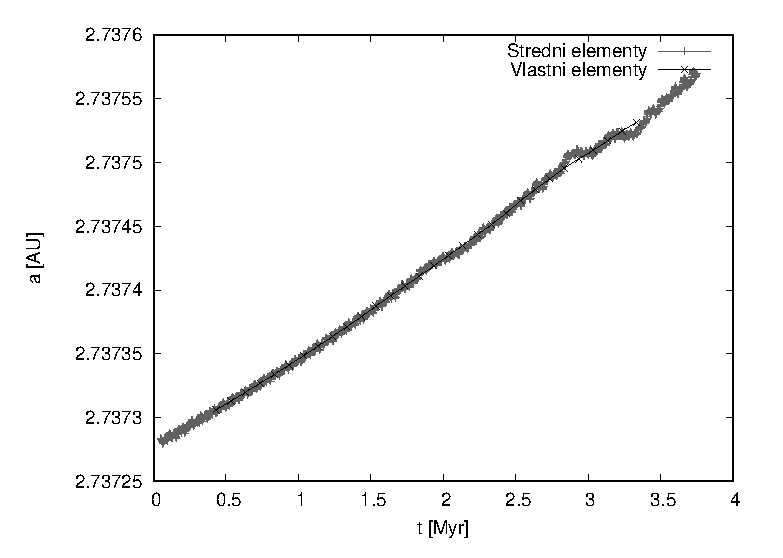
\includegraphics[width=0.8\textwidth]{obr/atFP}
	\caption{Porovnání střední $a_{\rm m}$ a vlastní $a_{\rm p}$ hlavní poloosy pro simluaci jedné planetky po dobu $3,76$ miliónů let. Lze vidět, že se za tuto dobu vlastní hlavní poloosa planetky zvýšila o~$\Delta a\doteq0.00022554\,{\rm AU}=33740,3\, {\rm km}$. Tento vývoj je způsobem Jarkovského jevem.}
	\label{atFP}
\end{figure}

Vlastní elementy jsou elementy dráhy zbavené jak krátkých, tak dlouhých periodických perturbací, mezi které kromě již zmíněných patří navíc sekulární rezonance, které jsou způsobeném závislostí frekvencí precese (změny) argumentu perihélia a délky vzestupného uzlu planetky a některé jiné planety nebo i vícero planet.

Vlastní elementy jsou tedy svým způsobem aritmetickými \uv{průměry} pohybu a jsou téměř neměnné na dlouhém časovém úseku, ačkoliv působením negravitačních sil --- především zmiňovaného Jarkovského jevu --- se můžou pomalu zvětšovat nebo zmenšovat. 

Mezi vlastní elementy počítáme pouze vlastní hlavní poloosu $a_{\rm p}$, vlastní excentricitu $e_{\rm p}$ a vlastní inklinaci $i_{\rm p}$. Ostatní elementy nemá cenu uvažovat, protože argument perihélia i délka vzestupného uzlu periodicky precedují (mění se v intervalu $0^\circ$ až $360^\circ$) a střední anomálie je také přibližně lineárně závislá na čase.

\cite{sidlichovsky96}

\chapter{Planetky ve sluneční soustavě}

\begin{figure}[!htb]
	\centering
	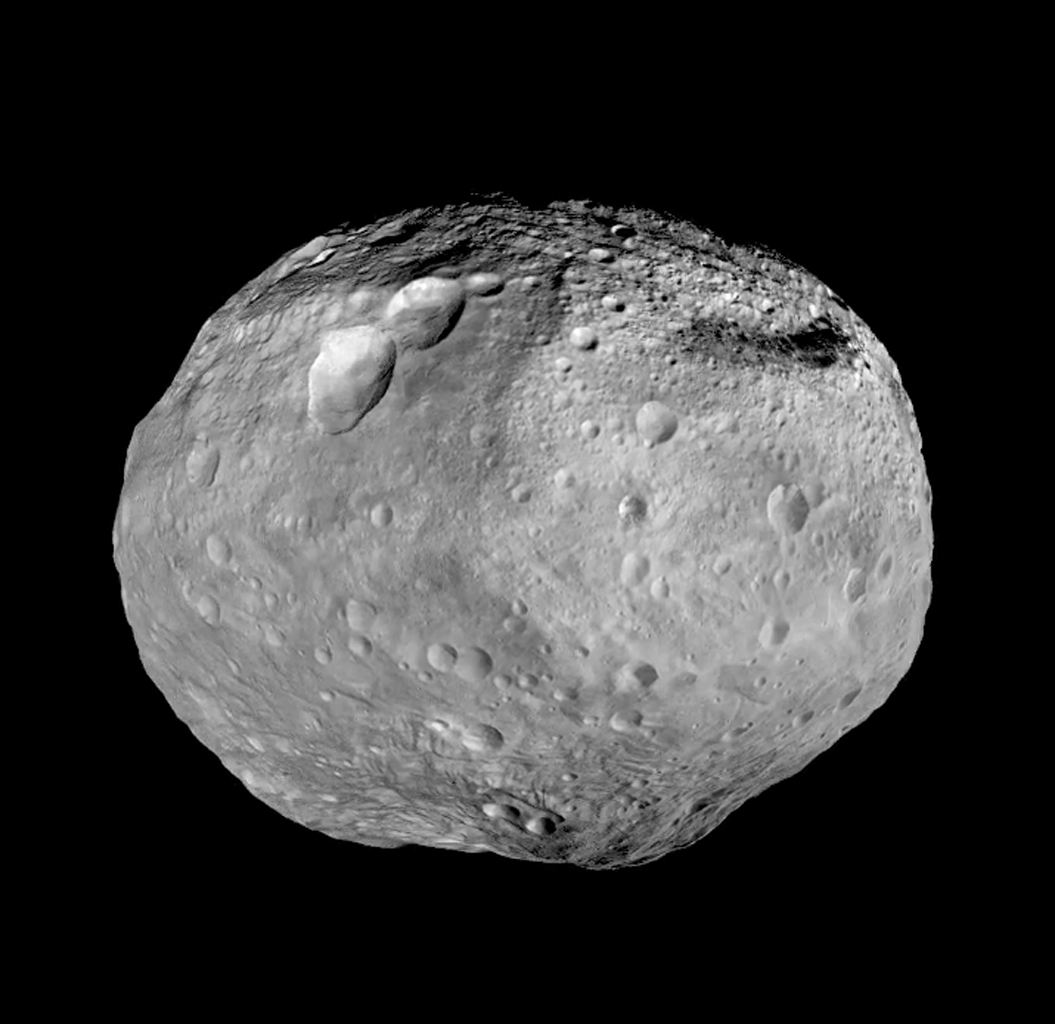
\includegraphics[width=0.7\textwidth]{obr/vesta.jpg}
	\caption{Planetka (4) Vesta, která je po trpasličí planetě (1) Ceres druhým největším a nejhmotnějším tělesem hlavním pásu planetek. Fotografie byla pořízena sondou \I{Dawn}, jejíž cílem byl i (1) Ceres. Zdroj: \cite{jplvesta}.}
\end{figure}

Podle Mezinárodní astronomické unie (IAU) se tělesa ve sluneční soustavě dělí hlavně na planety, komety, přirozené satelity a planetky. Planeta je definována jako takové těleso, které obíhá kolem Slunce, má dostatečnou hmotnost, aby si udrželo kulovitý tvar, a je \uv{vyčistilo} svoje okolí od ostatních těles. Kometa je těleso složené z~ledu a prachu, které většinou obíhá Slunce po velmi excentrické dráze a zanechává přitom za sebou ohon, který je způsoben vypařováním ledu z~komety působením slunečního záření. Dále přirozené satelity jsou tělesa obíhající nějakou planetu nebo planetku. 

\begin{figure}
	\centering
	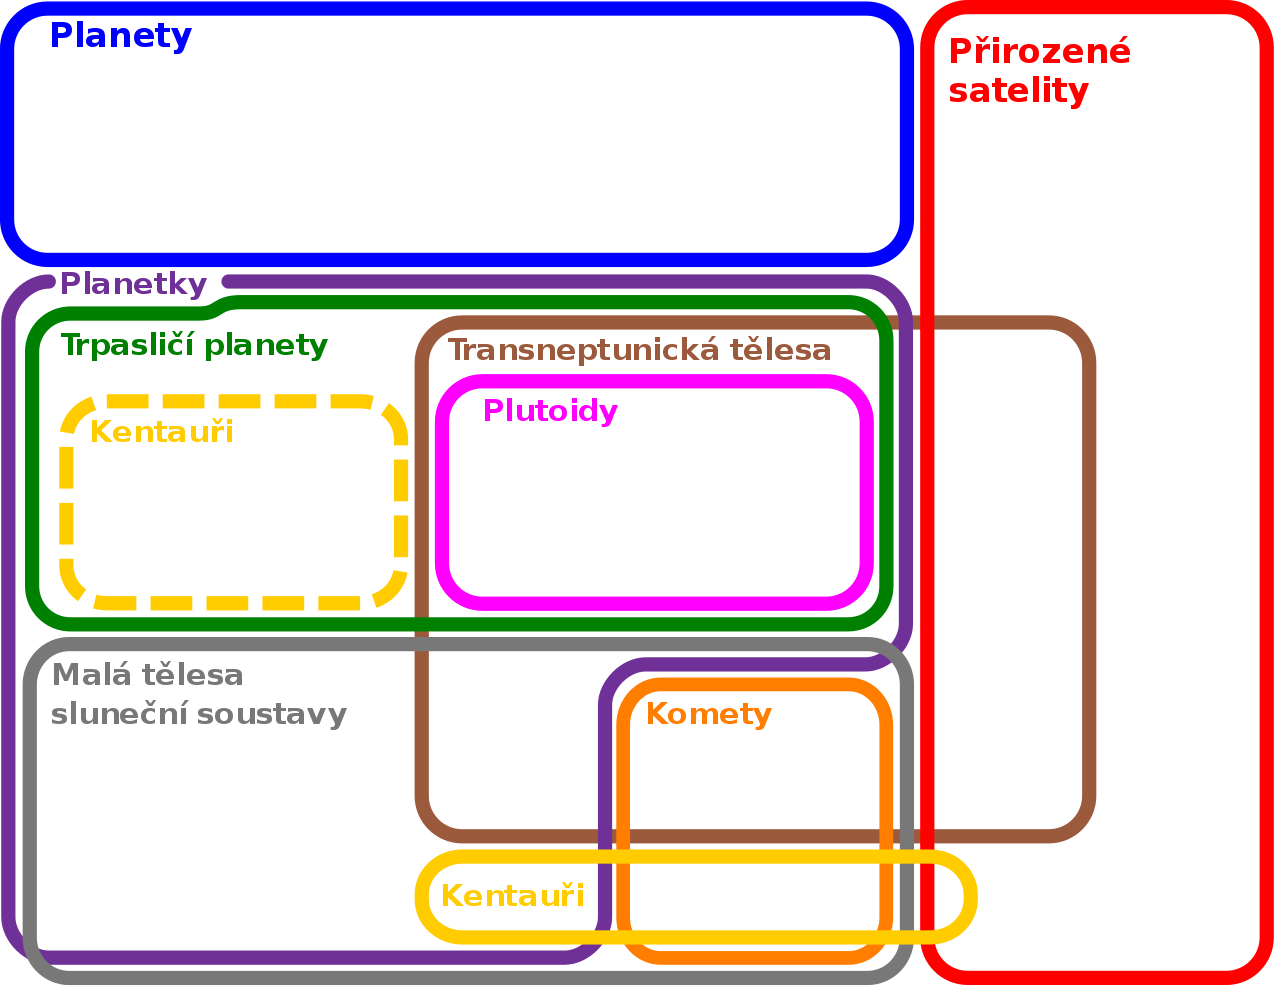
\includegraphics[width=0.6\textwidth]{obr/ssb.png}
	\caption{Zařazení těles sluneční soustavy podle IAU (po valném shromáždění v~Praze roku 2006, kde byl definován pojem planeta, čímž bylo vyřazeno Pluto z~planet sluneční soustavy.) Zdroj: \cite{wiki:ssb} \label{fig:ssb}}
\end{figure}

Konečně všechno ostatní je klasifikování jako planetka (někdy nepřesně označováno jako asteroid) --- patří sem trpasličí planety (těch je zatím pouze pět: Ceres, Pluto, Eris, Makemake, Haumea), transneptunická tělesa (tělesa, která se pohybují za oběžnou dráhou Neptunu), malá tělesa sluneční soustavy a další. Tyto skupiny se navzájem překrývají, viz~\ref{fig:ssb}. Dále můžeme planetky dělit na podle jejich oběžné dráhy na tělesa vnitřní a vnější sluneční soustavy. Většina těles vnější sluneční soustavy se nachází v~Kupierově pásu, který se sahá od oběžné dráhy Neptunu až do vzdálenosti přibližně $55\, {\rm AU}$. Tělesa vnitřní sluneční soustavy jsou přibližně omezená oběžnou dráhou Jupitera --- největší populace se nachází v~hlavním pásu, který se nachází mezi oběžnonou dráhou Marsu (přbližně $1,5\, {\rm AU}$) a Jupitera (přibližně $5,2\, {\rm AU}$). Dále sem spadají také planetky, jejichž oběžná dráhá protínu dráhu Marsu nebo Země --- blízkozemní planetky, a planetky nacházející se v~libračních centrech L4 a L5\footnote{To jsou takové body, v~nichž se vyrovnává působení gravitační a odstředivé síly. Jde tedy o~jakýsi bod rovnováhy. Body L4 a L5 se nachází na oběžné dráze většího tělesa o~$60^o$ \uv{napřed} nebo \uv{za} tělesem.} soustav Slunce--Země, Slunce--Mars, Slunce--Jupiter --- trojáni. Hildy???

\section{Hlavní pás planetek}

\begin{figure}
	\centering
	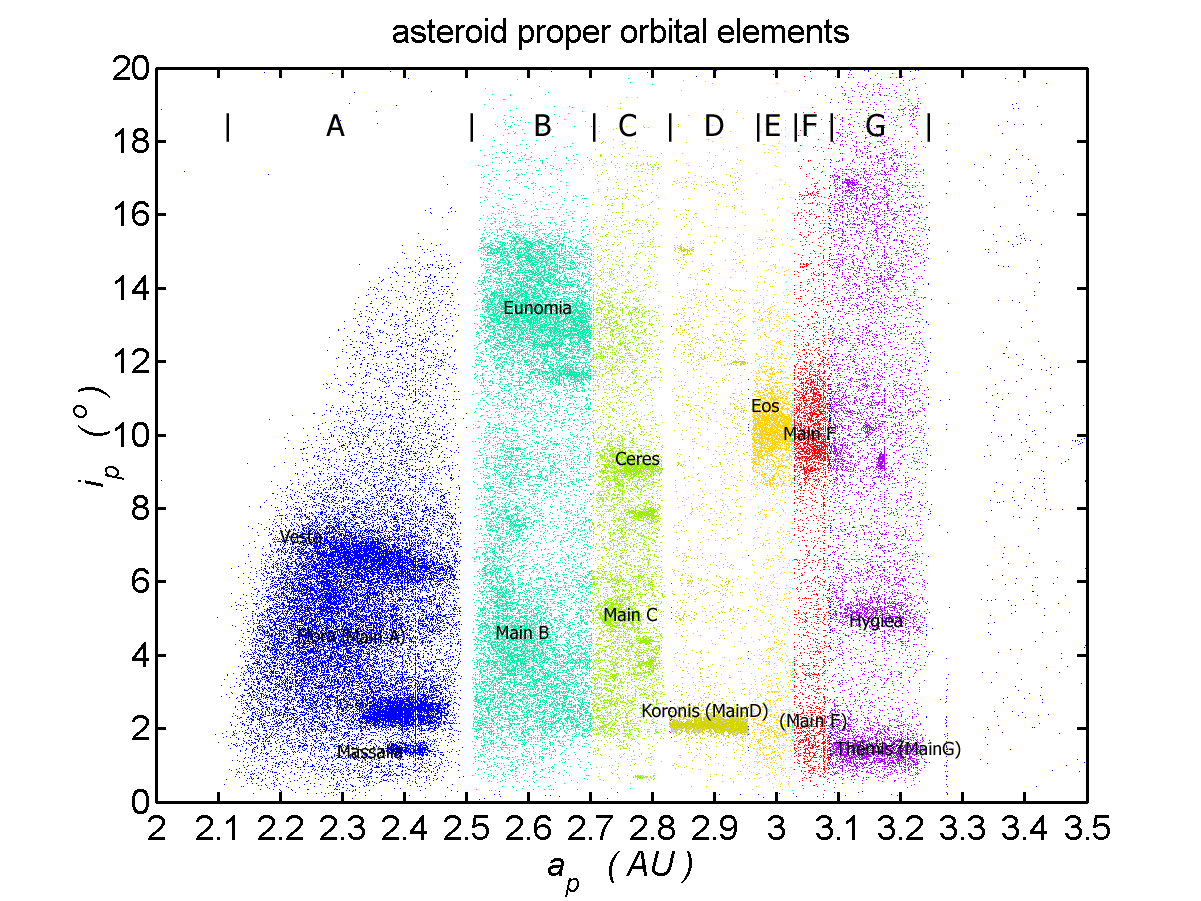
\includegraphics[width=0.8\textwidth]{obr/mainbelt.png}
	\caption{Planetky hlavního pásu podle vlastních elementů --- osa $x$ znázorňuje vlastní poloosu a osa $y$ vlastní sklon. Lze vidět některé rodiny planetek, konkrétně například uprostřed nahoře Eunomia. Barevné označení znázorňuje oblasti mezi rezonancemi středního pohybu.} \label{fig:belt}
\end{figure}

Při našem studiu se budeme zaměřovat na planetky hlavního pásu, ve kterém se také nachází jediná trpasličí planeta ve vnitřní sluneční soustavě Ceres, který má střední poloměr $473\, {\rm km}$. Ostatní planetky mají střední poloměr od $250\, {\rm km}$ po pouze několik metrů???. Největší populace se rovnoměrně rozprostírá od vzdálenosti $2,1\, {\rm AU}$ od Slunce do vzdálenosti přibližně $3,3\, {\rm AU}$. Planetky, které vystoupí z~této oblasti, se buď příblíží Marsu a jsou jeho gravitací vymrštěny na zcela odlišnou oběžnou dráhu, nebo se podobně přiblíží Jupiteru, který ji též může odklonit od původní oběžné dráhy nebo ji může zachytit ve svém gravitačním působení, čímž se planetka stane přirozenou družicí Jupitera. 

\section{Rezonance}
Struktura hlavního pásu planetek je významně ovlivněna rezonancemi, což jsou oblasti v~prostoru, ve kterém když se planetka nachází, je nějaký údaj o~její dráze a nějaké planety, běžně Jupitera nebu Saturnu, v~jednoduchém poměru, tedy ve zlomku s~nízkým čitatelem a jmenovatelem. Pro sekulární rezonance můžeme mít i složitější vztahy, kdy spolu porovnáváme více veličin zároveň. 
\subsection{Rezonance středního pohybu} \label{sec:meanmotion}
%Nástin výpočtu jejich polohy (je to jednoduché), vysvětlení vlivu na HCM

Rezonance středního pohybu jsou nejjednodušším, a zároveň také nejsilnějším typem rezonancí. Nastávají, když je oběžná doba planetky a planety v~poměru s~nízkými čísly, např. $3:2$ --- to znamená, že zatímco planetka dokončí tři celé oběhy, planeta vykoná dva a obě tělesa se znovu potkají na počáteční pozici. 

Vlivem těchto rezonancí se může hlavní poloosa planetky a excentricita periodicky měnit, podobně jako je tomu při kyvadlu. Některé rezonance naopak postupně zvyšují excentricitu dráhy planetky, až se její perihélium dostane pod oběžnou dráhu nějaké vnitřní planety, např. Marsu nebo Země, což eventuelně způsobí vzájemné blízké přiblížení, které planetku vymrští na úplně jinou oběžnou dráhu. Takto se planetka může stát blízkozemním objektem (\C{neo} --- Near--Earth object), součástí Kupierova pásu, který se nachazí za orbitou Neptunu nebo může být úplně vystřelena ze sluneční soustavy. Za vhodných podmínek se perihélium planetky může snížit natolik, že překročí Rocheovu mez\footnote{což je hraniční vzdálenost od centrálního tělesa, kterou když planetka držená pohromadě vlastní gravitací překročí, je vlivem slapových jevů roztržena na malé kousky.} a je později pohlcena hvězdou a stává se její součastí \cite{pichierri17}.

Výpočet umístění rezonance středního pohybu, tedy vzdálenosti od Slunce, je poměrně jednoduchý, uvádíme proto postup pro rezonanci ovlivňující rodinu Eunomia, kterou je rezonance $8:3$ s~Jupiterem.

Vzpomeňme na Třetí Keplerův zákon, který říká
\begin{align} \label{eq:3kep}
	\frac{T_1^2}{T_2^2}=\frac{a_1^3}{a_2^3}, 
\end{align}
kde $T_1$, $T_2$ označují oběžné dvou tělesa a $a_1$, $a_2$ jejich hlavní poloosy. 

Předpokládejme, že v~námi hledané rezonanci $8:3$ se nachází nějaká planetka a vypočítejme délku její hlavní poloosy, a to úpravou rovnice~\eqref{eq:3kep} jako
\begin{align} \label{eq:3kepa}
	a_2=\left(\frac{T_2}{T_1}\right)^{\frac{3}{2}}a_1
\end{align}
kde $T_1$, resp.\ $T_2$ v~tomto značí oběžnou dobu Jupitera, resp.\ planetky, a $a_1$, resp.\ $a_2$ délku hlavní poloosy Jupitera, resp.\ planetky. Oběžná doba Jupitera je přibližně $4332,59\,$dnů a délka jeho hlavní poloosy je přibližně $5,203\,{\rm AU}$. Protože hledáme rezonanci $8:3$, musí platit $\frac{T_2}{T_1}=\frac{3}{8}$. Po dosazení do rovnice~\eqref{eq:3kepa} dostáváme $a_2=2.706\,{\rm AU}$, což lze dobře ověřit na obrázku~\ref{fig:ae_ai_wise} rozdělení rodiny Eunomia v~prostoru hlavní poloosy a excentricity nebo sklonu v~pozdější kapitole~\ref{ch:eunomia}.
\subsection{Sekulární rezonance} 
Sekulární rezonance jsou mnohem mírnějšího rázu než rezonance středního pohybu, ale na dlouhodobý vývoj hlavního pásu mají velký vliv. Slovo sekulární pochází z~latinského \I{saeculum}, což znamená století nebo generace, což ukazuje na dlouhodobý charakter sekulárních rezonancí. Veličiny, které zde dáváme do poměru, jsou rychlosti precese argumentu perihélia a rychlosti precese délky vzestupného uzlu. 
\section{Rodiny planetek}


Definice --- katastrofická srážka, rozptýlení ve střední anomálii, podobnost pouze ve vlastních elementech, přesunout sem kapitoly o~Jarkovského jevu, YORPu a náhodných srážkách???

Rodiny planetek jsou skupiny vesmírných těles, mající podobné charakteristiky, předně ve vlastních elementech dráhy. Při jejich identifikaci musíme ale přihlížet i na ostatní veličiny, jako jsou albedo, barevné indexy, nebo odhadované složení. 

\begin{figure}
	\centering
	\includegraphics[width=0.49\textwidth]{obr/trajec_001.png}
	\includegraphics[width=0.49\textwidth]{obr/trajec_101.png} \\
	\includegraphics[width=0.49\textwidth]{obr/trajec_201.png}
	\includegraphics[width=0.49\textwidth]{obr/trajec_501.png}
	\caption{Trojrozměrný vzhled rodiny Eunomia v~časech $t=0,\,10000,\,20000,\,50000\,{\rm let}$ po úvodním izotropním rozpadu. Lze pozorovat rozprostření ve střední anomálii.} \label{fig:trajec}
\end{figure}

Vznikají srážkou dvou planetek, čemuž v~závislosti na poměru velikosti mateřského (největšího) tělesa říkáme buď \I{katastrofický rozpad} (\uv{na malé kousíčky}), nebo \I{kráterování}. Může se zdát, že takové srážky jsou v~tak velkém prostoru jako je sluneční soustava velmi málo pravděpodobné, ale v~dlouhém časovém úseku --- $4,5\,\text{miliardy let}$ od vzniku naší sluneční soustavy --- k~srážkám dochází, a mají nejenom vliv na vznik rodin, ale také na jejich následný vývoj (vzniklé fragmenty se spolu nadále sráží).


Rodiny planetek, které již prošly dlouhodobým vývojem, se na obloze nejeví jako skupinka společně letících planetek, kvůli rozdílné oběžné době se totiž rozptýlí ve střední anomálii, jak lze vidět na obrázku~\ref{fig:trajec}.

\subsection{Metody identifikace rodin}
Nejpoužívanější metodou pro identifikaci rodin planetek je \I{hierarchická shlukovací metoda} (HCM) \cite{zappala90}. Spočívá v tom, že si v trojrozměrném prostoru vlastních elementů ($a_{\rm p},\,e_{\rm p},\,i_{\rm p}$) zvolíme metriku --- veličinu, kterou budeme popisovat \uv{vzdálenost} dvou těles, a poté, pomocí zvolené hraniční velikosti této metriky, určíme, která tělesa \uv{patří k sobě}. Tato metrika má jednotku rychlosti, lze totiž ukázat, že se v podstatě jedná o únikovou rychlost tělesa od mateřského tělesa při rozpadu. Je určena vztahem
\begin{align}
	v=na_{\rm p}\sqrt{C_a\left(\frac{\Delta a_{\rm p}}{a_{\rm p}}\right)^2+C_e(\Delta e_{\rm p})^2+C_i(\Delta \sin i_{\rm p})^2}\,,
\end{align}
kde $n$ značí střední pohyb, dále pokud označíme $1$ a $2$ tělesa, mezi kterými metriku počítáme, platí $a_{\rm p}=(a_{{\rm p}1}+a_{{\rm p}2})/2$ a $\Delta a_{\rm p}=a_{{\rm p}1}-a_{{\rm p}2}$, $\Delta e_{\rm p}=e_{{\rm p}1}-e_{{\rm p}2}$ a $\Delta \sin i_{\rm p}=\sin i_{{\rm p}1}-\sin i_{{\rm p}2}$, $C_a,\,C_e,\,C_i$ jsou váhy, které přirazujeme jednotlivým elementům, přičemž možnou a i v této práci použitou volbou je $C_a=5/4$, $C_e=2$, $C_i=2$. 

Samotný průběh tohoto algoritmu je pak jednoduchý: zvolíme nějakou hraniční rychlost $v_{\rm cutoff}$ a poté, většinou počínaje největším tělesem, např. (15) Eunomia, hledáme dvojice těles, pro které je $v<v_{\rm cutoff}$; vždy když nějakou nalezneme, přidáme si ji do seznamu zkoumané rodiny a postup opakujeme, dokud nám nepřibývají žádní noví členové. Výsledný počet členů je samozřejmě závislý na volbě $v_{\rm cutoff}$, což lze vidět na obrázku~\ref{fig:Nv}.

Jak ukážeme později v této práci, tato metoda samotná nestačí ke kompletní identifikaci rodiny, neboť musíme odstranit \I{přimíšená tělesa} (\I{interlopers}) porovnáním albed (viz obráze~\ref{fig:pV_pIR}), barevných indexů (viz obrázek~\ref{fig:astar_iz}), grafu závisloti hlavní poloosy a hvězdné velikosti nebo dalšími metodami. 

\subsection{Nevratné děje při vývoji}
Disipační síly, vliv na vývoj v~prostoru vlastních elementů, reference na nějaký článek o~nové databázi tvarů planetek???
\subsubsection{Jarkovského jev} \label{sec:jarko}
Popis, vysvětelní obrázku aH, vliv na vlastní elementy, účinky kolem rezonancí
\begin{figure}[!htb]
	\centering
	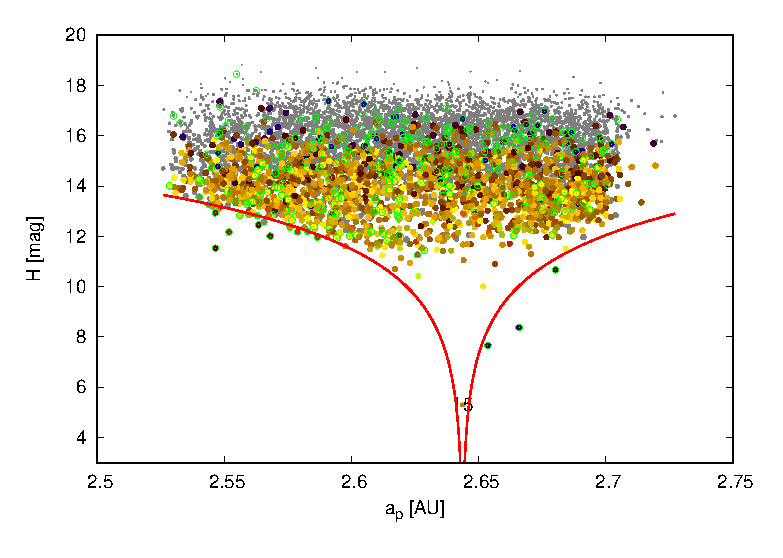
\includegraphics[width=0.5\textwidth]{obr/aH_wise}
	\caption{Rozdělení pozorované rodiny Eunomia v~rovině vlastní hlavní poloosy $a_p$ a absolutní hvězdné velikosti $H$. Lze pozorovat typický tvar \uv{V}, který je způsobem počátečním rychlostním polem a Jarkovského jevem, který je navíc ještě zesílen vlivem YORPu, což způsobuje zvýšenou koncentraci malých planetek na okrajích rodiny.}
	\label{aH_wise}
\end{figure}
\subsubsection{YORP jev}
Popis, zmínka o~Poynting–Robertson efektu???, zesílení Jarkovského jevu
\subsubsection{Náhodné srážky}
???

\chapter{Vlastnosti rodiny Eunomia} \label{ch:eunomia}
Postup určování rodiny, volba $v_{cutoff}$, pozadí --- [česky???] interlopers (ref na později), rozdělení velikostí 
\begin{figure}[!htb]
	\centering
	\includegraphics[width=0.6\textwidth]{obr/Nv}
	\caption{Závislost počtu členů rodiny Eunomia na zvolené hraniční rychlosti $v_{\rm cutoff}$ při výpočtu HCM. Počet členů prudce vzroste při přechodu z~rychlosti $43\,{\rm m/s}$ na $44\,{\rm m/s}$, což je způsobené poměrně velkou vzdáleností prvního nejbližšího tělesa od mateřského (15) Eunomia. Dále vzroste prudce při přechodu z~rychlosti $46\,{\rm m/s}$ na $47\,{\rm m/s}$, což je způsobené splynutím s~rodinou Adeona.}
	\label{Nv}
\end{figure}
\begin{figure}[!htb]
	\centering
	\begin{subfigure}[b]{0.45\textwidth}
	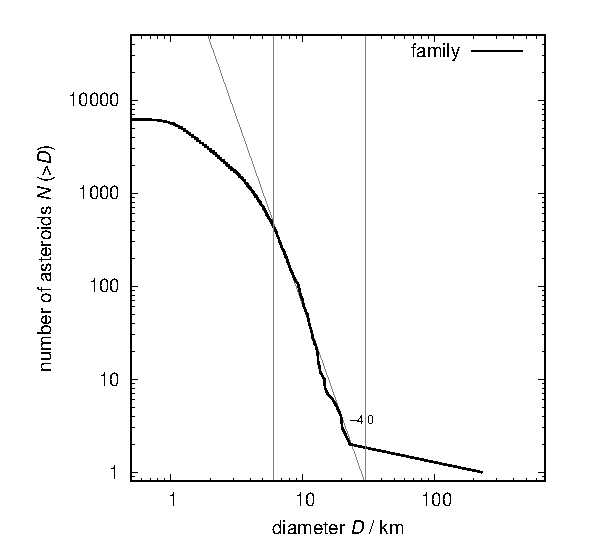
\includegraphics[width=\textwidth]{obr/size_distribution}
	\end{subfigure}
	\begin{subfigure}[b]{0.45\textwidth}
	\includegraphics[width=\textwidth]{obr/size_distribution_SMALLD}
	\end{subfigure}
	\caption{Histogram četnosti velikostí planetek rodiny Eunomia, kde veličina $N({>}D)$ označuje počet planetek s~průměrem větším než $D$.}
	\label{size_distribution}
\end{figure}
\section{Fyzikální model pro rodinu Eunomia}
Rozdělení v~$ae$ a $ai$ prostoru, vliv rezonancí J8/3 a J13/5, Gaussovy rovnice --- elipsa, volba bodu rozpadu ($f=90^o$, $\omega+f=50^o$).
\begin{figure}[!htb]
	\centering
	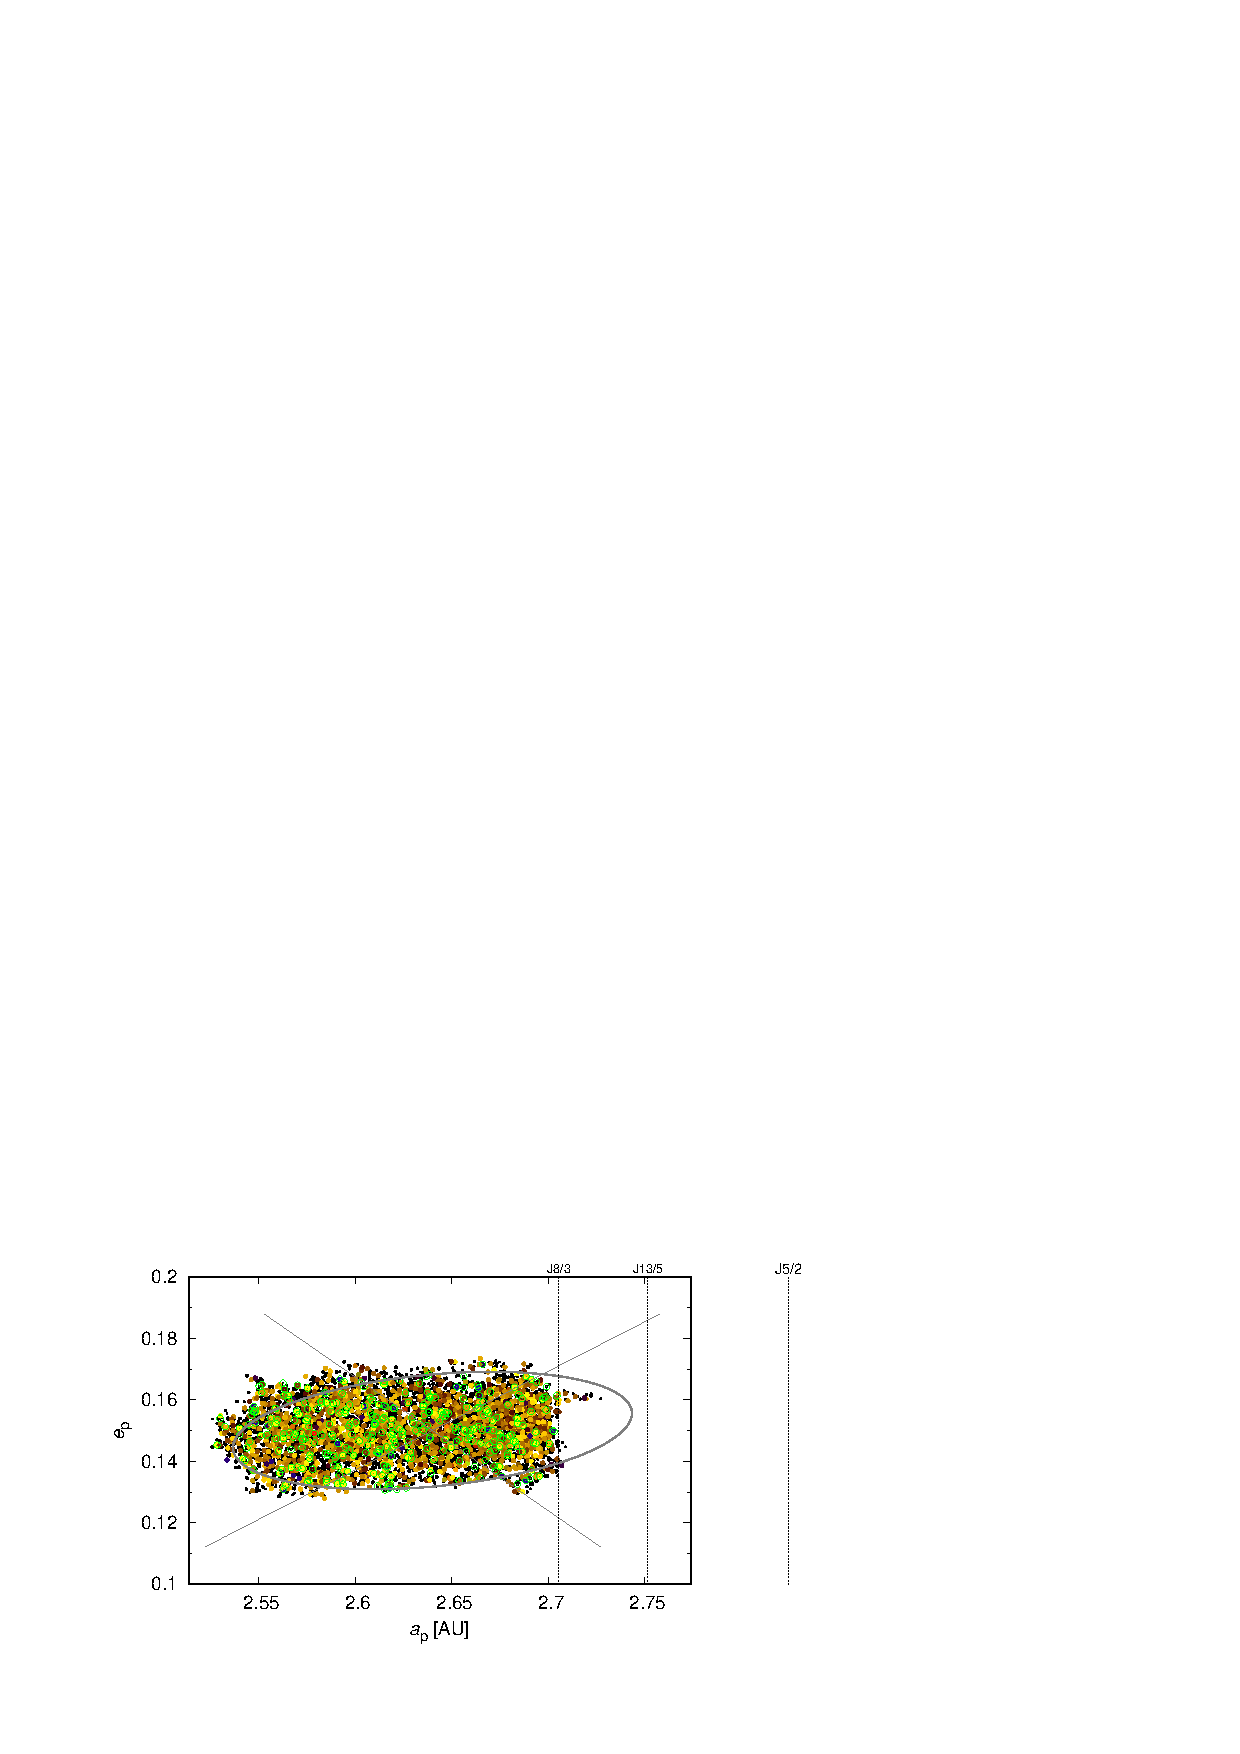
\includegraphics[width=0.7\textwidth]{obr/ae_wise}
	\includegraphics[width=0.7\textwidth]{obr/ai_wise}
	\caption{Pozorovaná rodina Eunomia v~rovině vlastní hlavní poloosy $a_{\rm p}$ a vlastní excentricity $e_{\rm p}$ (nahoře) a v~rovině vlastní hlavní poloosy $a_{\rm p}$ a vlastního sklonu $\sin i_{\rm p}$ (dole). Barevná škála odpovídá albedu $p_V$ a $p_IR$ z~katalogu WISE. Nápisy J8/3 a J13/5 označují polohu rezonancí středního pohybu s~Jupiterem. Šedé elipsy a úsečky naznačují výpočet Gaussových rovnic pro hodnoty pravé anomálie $f=0^\circ,\,90^\circ,\,180^\circ$ a $\omega+f=0^\circ,\, 50^\circ,\, 90^\circ$, kde zvolenou hodnotou je $f=90^\circ$ a $\omega+f=50^\circ$.}
	\label{fig:ae_ai_wise}
\end{figure}
\subsubsection{Přimíšená tělesa}
Odstranění interlopers, barevné indexy, SLOAN, WISE, ref na Nejistoty veřejných dat.
\begin{figure}[!htb]
	\centering
	\includegraphics[width=0.7\textwidth]{obr/pV_pIR}
	\caption{Albeda $p_V$ a $p_{IR}$ z~katalogu WISE \cite{nugent15}. Pro vyřazení přimíšených byly zvoleny hraniční hodnoty $0.05 \leq p_v \leq 0.4$.}
	\label{fig:pV_pIR}
\end{figure}
\begin{figure}[!htb]
	\centering
	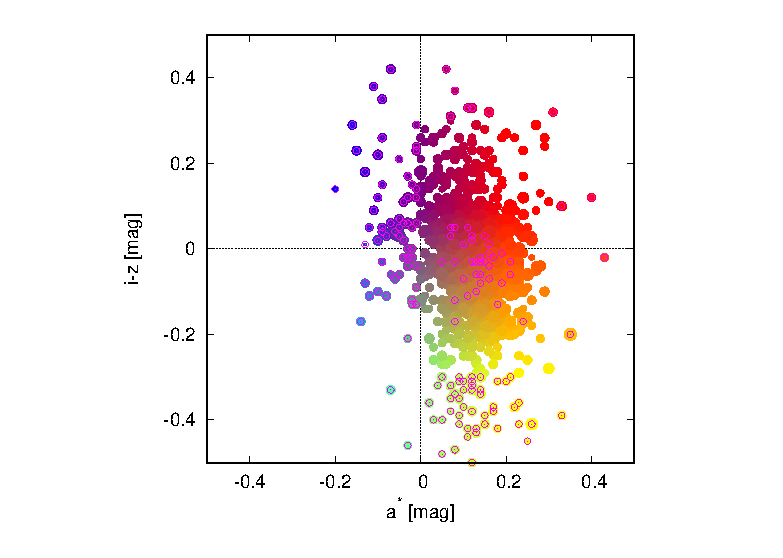
\includegraphics[width=0.7\textwidth]{obr/astar_iz}
	\caption{Barevné indexy $a^*$ a $i-a$ z~katalogu SLOAN \cite{ivezic01}. Pro vyřazení přimíšených těles byly zvoleny hraniční hodnoty $0\leq a^* \leq 0.3$ a $-0.3\leq i-z \leq 0.3$.}
	\label{fig:astar_iz}
\end{figure}
\section{Nejistoty pozorovaných dat}
???

Následující dvě kapitoly budou napsány až po doběhnutí simulace. 
\section{(Simulace orbitálního vývoje)}
\subsection{(Dlouhodobé simulace)}
Popis experimentu (údaje o~výpočetní technice)
\section{(Porovnání modelu a pozorování)}

\chapter{Budoucí možnosti výzkumu}
???

\newpage

\printbibliography

\begin{appendices}
	\chapter{Výpočet Keplerovy rovnice pomocí iterační metody} \label{app:kepit}
	May--Do: komentář
\begin{lstlisting}[language=Python]
def kepler(M, e):
    """Solution of Kepler equation"""
    eps = 1E-13
    E2 = M+e*sin(M)
    while True:
        E1 = E2
        E2 = M+e*sin(E1)
        if abs(E2-E1)<eps:
            break 
    return E2
\end{lstlisting}
	\chapter{Výpočet polohy tělesa z oskulačních elementů} \label{app:el2xyz}
	May--Do: komentář
	\begin{lstlisting}[language=Python]
def el2xyz(path):
    """Conversion from orbital elements to xyz positions (from file bin.out by script follow2)"""
    binout = open(path, 'r')
    line = binout.readline()
    while line:
        elms = line.split()
        if int(elms[0]) > 0:
            a = float(elms[2])
            e = float(elms[3])
            inc = radians(float(elms[4]))
            capom = radians(float(elms[5]))
            omega = radians(float(elms[6]))
            M = radians(float(elms[7]))
    
            # E = M + (e-pow(e,3.0)/8.0)*sin(M) + pow(e,2)/2.0*sin(2.0*M) + pow(e,3)*3.0/8.0*sin(3.0*M)
            E = kepler(M, e)
            f = 2.0*atan(sqrt((1.0+e)/(1.0-e))*tan(E/2.0))
            r = a*(1-e*cos(E))
            x = r*(cos(capom)*cos(omega+f)-sin(capom)*sin(omega+f)*cos(inc))
            y = r*(sin(capom)*cos(omega+f)+cos(capom)*sin(omega+f)*cos(inc))
            z = r*sin(inc)*sin(omega+f)
            print (str(elms[1]) + " " + str(x) + " " + str(y) + " " + str(z))
        line = binout.readline()
	\end{lstlisting}
\end{appendices}
\end{document}
